\documentclass[]{article}
\usepackage{lmodern}
\usepackage{amssymb,amsmath}
\usepackage{ifxetex,ifluatex}
\usepackage{fixltx2e} % provides \textsubscript
\ifnum 0\ifxetex 1\fi\ifluatex 1\fi=0 % if pdftex
  \usepackage[T1]{fontenc}
  \usepackage[utf8]{inputenc}
\else % if luatex or xelatex
  \ifxetex
    \usepackage{mathspec}
    \usepackage{xltxtra,xunicode}
  \else
    \usepackage{fontspec}
  \fi
  \defaultfontfeatures{Mapping=tex-text,Scale=MatchLowercase}
  \newcommand{\euro}{€}
    \setmainfont{Helvetica Neue}
\fi
% use upquote if available, for straight quotes in verbatim environments
\IfFileExists{upquote.sty}{\usepackage{upquote}}{}
% use microtype if available
\IfFileExists{microtype.sty}{%
\usepackage{microtype}
\UseMicrotypeSet[protrusion]{basicmath} % disable protrusion for tt fonts
}{}
\usepackage{graphicx}
\makeatletter
\def\maxwidth{\ifdim\Gin@nat@width>\linewidth\linewidth\else\Gin@nat@width\fi}
\def\maxheight{\ifdim\Gin@nat@height>\textheight\textheight\else\Gin@nat@height\fi}
\makeatother
% Scale images if necessary, so that they will not overflow the page
% margins by default, and it is still possible to overwrite the defaults
% using explicit options in \includegraphics[width, height, ...]{}
\setkeys{Gin}{width=\maxwidth,height=\maxheight,keepaspectratio}
\ifxetex
  \usepackage[setpagesize=false, % page size defined by xetex
              unicode=false, % unicode breaks when used with xetex
              xetex]{hyperref}
\else
  \usepackage[unicode=true]{hyperref}
\fi
\hypersetup{breaklinks=true,
            bookmarks=true,
            pdfauthor={},
            pdftitle={Sample Report},
            colorlinks=true,
            citecolor=blue,
            urlcolor=blue,
            linkcolor=magenta,
            pdfborder={0 0 0}}
\urlstyle{same}  % don't use monospace font for urls
\setlength{\parindent}{0pt}
\setlength{\parskip}{6pt plus 2pt minus 1pt}
\setlength{\emergencystretch}{3em}  % prevent overfull lines
\setcounter{secnumdepth}{0}

\title{Sample Report\\\vspace{0.5em}{\large M.Kaller\_14\_05 - P1170\_101}}
\date{2014-11-19}

\begin{document}
\maketitle

\section{Sample Information}\label{sample-information}

\begin{description}
\item[Report Date]
2014-11-13
\item[Recipient]
phil.ewels@scilifelab.se
\item[Project Name]
M.Kaller\_14\_05
\item[User Sample Name]
Test Sample \#1290
\item[NGI Sample Name]
P1170\_101
\item[Library Preparation Method]
\textbf{A:} All samples were sequenced on HiSeq2500 (HiSeq Control
Software 2.0.12.0/RTA 1.17.21.3) with a 2x101 setup.The Bcl to Fastq
conversion was performed using bcl2Fastq v1.8.3 from the CASAVA software
suite. The quality scale used is Sanger / phred33 / Illumina 1.8+.
\item[Sequencing Centre]
NGI Stockholm
\item[Sequencing Platform]
Illumina
\item[Reference Genome]
\texttt{gatk\_bundle/2.8/b37/human\_g1k\_v37.fasta}
\item[Flow Cells]
\texttt{140815\_SN1025\_0222\_BC4HAPACXX}

\texttt{140815\_SN1025\_0223\_BC4HAPACXX}
\end{description}

\section{Library Statistics}\label{library-statistics}

\begin{description}
\itemsep1pt\parskip0pt\parsep0pt
\item[Total Reads]
908,585,160
\item[Aligned Reads]
99.47\% - 903,806,933
\item[Duplication Rate]
1.9\%
\item[Median Insert Size]
369 bp
\item[Av. Autosomal Coverage]
28.92
\item[Reference with at least 30X Coverage]
51.72\%
\item[GC Content]
39.87\%
\end{description}

See below for more information about coverage and insert size. The
\texttt{qualimapReport.html} report in your delivery folder contains
additional library statistics. Note that the duplication rate above is
calculated using
\href{http://broadinstitute.github.io/picard/command-line-overview.html\#MarkDuplicates}{Picard
Mark Duplicates}. Qualimap calculates duplicates differently and the
figure in the report will be different to the Picard result..

\subsection{Distribution of sequencing
coverage}\label{distribution-of-sequencing-coverage}

Calculating the coverage of a genome tells you how much information you
have about the sequence content of any given position. More coverage
means more data and so greater confidence in your results. A specific
locus with 30X coverage will have 30 unique reads covering that
location. Different positions in the genome may have different coverages
due to variations in how well reads map to the underlying sequence.
Other factors such as GC bias in library preparation may also have an
effect.

To calculate the plot below, we create rolling windows across the genome
and count the frequencies of the different coverages observed. This was
done using the \href{http://qualimap.bioinfo.cipf.es/}{QualiMap} tool
and plotted with an
\href{https://github.com/SciLifeLab/visualizations}{NGI script}.

\begin{figure}[htbp]
\centering
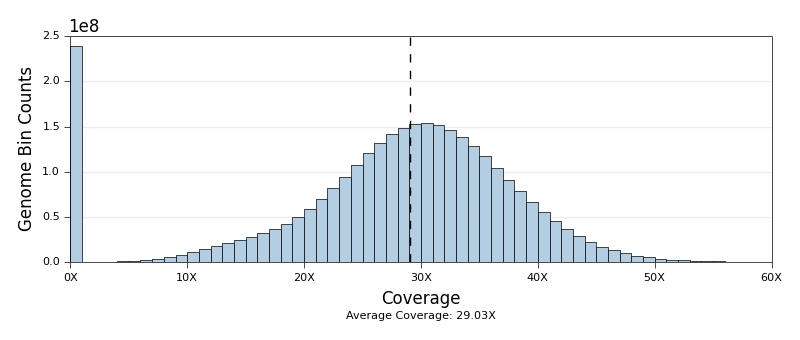
\includegraphics{plots/qualimap_coverage.png}
\caption{Sequencing Coverage}
\end{figure}

\subsection{Proportion of library with increasing coverage
depths}\label{proportion-of-library-with-increasing-coverage-depths}

Another way to assess coverage is to look at the proportion of the
reference genome with a certain coverage. The plot below shows what
percentage of the reference genome is covered with increasing coverage
thresholds. As above, this data was calculated using
\href{http://qualimap.bioinfo.cipf.es/}{QualiMap} and plotted with an
\href{https://github.com/SciLifeLab/visualizations}{NGI script}.

\begin{figure}[htbp]
\centering
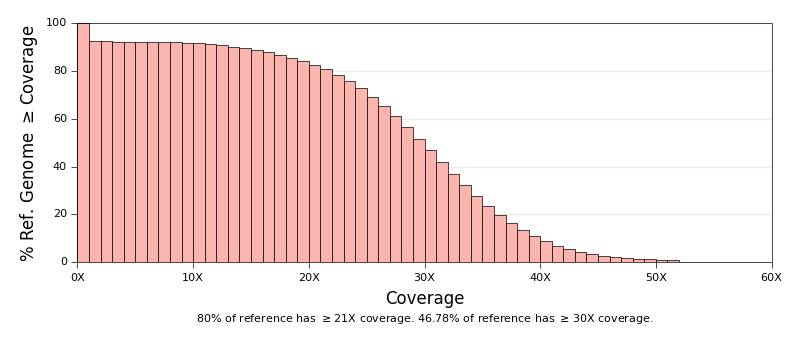
\includegraphics{plots/genome_fraction.png}
\caption{Genome Fractional Coverage}
\end{figure}

\subsection{Library fragment insert
sizes}\label{library-fragment-insert-sizes}

By inspecting where each read pair maps to in the reference genome, we
can reconstruct the reads that were present in the library and calculate
the range of insert sizes. This gives an insight into the quality of the
sequencing library. We counted how many reads with each insert size were
seen and plotted this in the histogram below. This was done using the
\href{http://qualimap.bioinfo.cipf.es/}{QualiMap} tool and plotted with
an \href{https://github.com/SciLifeLab/visualizations}{NGI script}.

\begin{figure}[htbp]
\centering
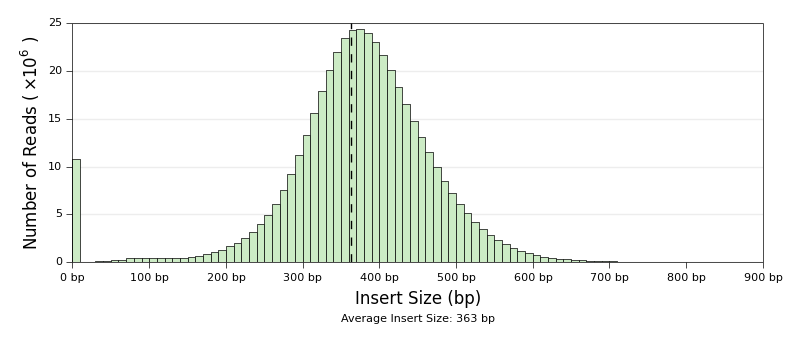
\includegraphics{plots/qualimap_insertsize.png}
\caption{Insert Sizes}
\end{figure}

\subsection{Distribution of reads by GC
content}\label{distribution-of-reads-by-gc-content}

Library preparation and sequencing alignment can be affected by
differences in GC content. Here, we plot the proportions of the library
reads at each GC content. The red dotted line shows the profile for the
reference genome. This data was calculated using
\href{http://qualimap.bioinfo.cipf.es/}{QualiMap} and plotted with an
\href{https://github.com/SciLifeLab/visualizations}{NGI script}.

\begin{figure}[htbp]
\centering
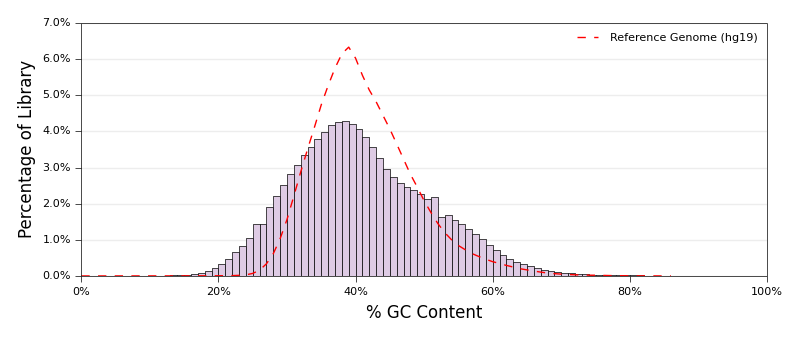
\includegraphics{plots/gc_distribution.png}
\caption{GC Content Distribution}
\end{figure}

\section{Variants}\label{variants}

\begin{description}
\itemsep1pt\parskip0pt\parsep0pt
\item[Change Rate]
1 change per 774 bp
\item[Total SNPs]
4,004,647
\item[Homotypic SNPs]
1,491,592
\item[Heterotypic SNPs]
2,513,055
\item[Transitions / Transversions Ratio]
1.9895
\item[Synonymous / Non-Synonymous]
35,078 / 30,232
\item[Stop Gained / Lost]
273 / 58
\item[Missense SNPs]
46.2\% - 30,366
\item[Nonsense SNPs]
0.4\% - 273
\item[Silent SNPs]
53.4\% - 35,078
\end{description}

Different effects can be attributed to each SNP depending on where it
occurs. Here we have used the
\href{http://snpeff.sourceforge.net/}{snpEff} tool to categorise and
count different effects. The results were plotted with an
\href{https://github.com/SciLifeLab/visualizations}{NGI script}.

\begin{figure}[htbp]
\centering
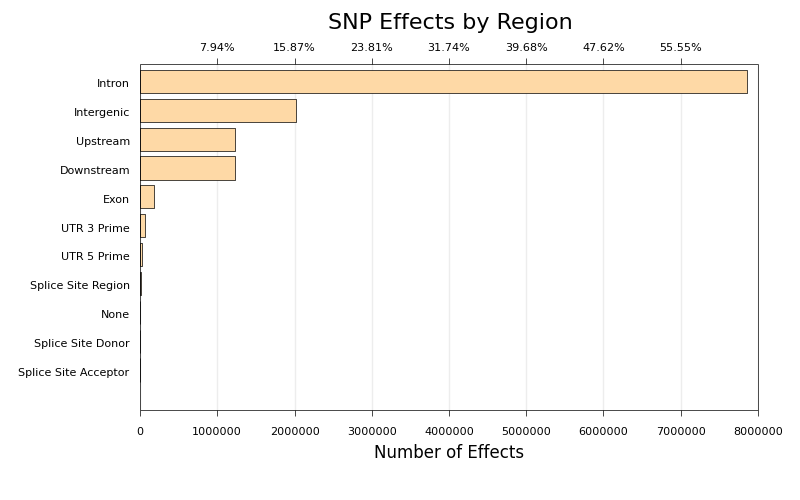
\includegraphics{plots/snpEff_effect_regions.png}
\caption{Insert Sizes}
\end{figure}

See the \texttt{snpEff\_summary.html} report in your delivery folder for
more details.

\end{document}
